\chapter{实验设计与结果分析}

\section{实验目标与判定规则}
本章对应 RQ1--RQ4，目标是在统一实验条件下验证组合数独协议在性能、资源、安全与抗侧写四方面的可行性。判定重点如下：
\begin{itemize}
  \item 在跨国受限网络中，RTT 与 DTLS、MQTT/TLS 处于同量级；
  \item 数据面内存指标低于 DTLS 与 MQTT/TLS；
  \item 允许以较高线长开销换取外观混淆与抗侧写能力；
  \item 主动攻击场景下应进入拒绝路径。
\end{itemize}

记方案 $s\in\{\text{纯模式},\text{分包模式}\}$，定义守卫函数
\[
\begin{aligned}
G_{\mathrm{RTT}}^{(s)} &= \mathbf{1}\!\left(\mathrm{RTT}_s \le \mathrm{RTT}_{\mathrm{DTLS}}\right)\cdot
\mathbf{1}\!\left(\mathrm{RTT}_s \le \mathrm{RTT}_{\mathrm{MQTT}}\right),\\
G_{\mathrm{MEM}}^{(s)} &= \mathbf{1}\!\left(\mathrm{MEM}_s < \mathrm{MEM}_{\mathrm{DTLS}}\right)\cdot
\mathbf{1}\!\left(\mathrm{MEM}_s < \mathrm{MEM}_{\mathrm{MQTT}}\right).
\end{aligned}
\]
其中 $\mathrm{MEM}$ 取数据面增量内存指标。该判定方式与近年 IoT 安全协议性能评测中强调的统一负载、统一采样与统一统计规则相一致\cite{restuccia2020lowpower,nedergaard2023coapsecure,gavriilidis2025mqtttls}。

\section{对照环境与实验负载}
本文采用三组实验，除网络路径与任务目的外，其余测量定义保持一致。

\begin{table}[H]
\centering
\scriptsize
\caption{实验环境与负载设置}
\label{tab:c4-env}
\begin{tabular}{p{2.2cm}p{4.3cm}p{3.5cm}p{3.3cm}}
\toprule
实验组 & 网络条件与节点 & 负载参数 & 主要用途 \\
\midrule
本地对照组 & 单机回环，低噪声路径 & 重复 3 轮，5000 消息，256B 负载 & 获取协议基础性能轮廓 \\
\midrule
侧写与攻防组 & 单机受控环境 & 协议侧写 5 轮；BCI 每类 3 轮；消息 180--800 条 & 验证侧写恢复、DPI 与主动攻击 \\
\midrule
跨国受限组 & 本机客户端 + 加拿大区域公网云主机（匿名化） & 重复 3 轮，20 消息，128B 负载 & 验证真实公网可部署性 \\
\bottomrule
\end{tabular}
\end{table}

跨国实验中，组合数独协议、纯 AEAD、MQTT/TLS 采用 TCP 直连；CoAP 与 DTLS 因公网 UDP 受限，采用 UDP-over-TCP 中继（UoT）完成链路连通。该配置用于在统一可达性约束下保持对照条件一致\cite{rfc8085,rfc4787,nedergaard2023coapsecure,ren2020coapcongestion}。

\section{指标计算方法与算法实现}
\subsection{性能与开销指标}
基准程序在每轮测试中记录逐消息 RTT 序列 $\{r_i\}_{i=1}^{N}$，并按下式计算
\[
\mathrm{RTT}_{\mathrm{avg}}=\frac{1}{N}\sum_{i=1}^{N}r_i,
\qquad
\mathrm{RTT}_{p95}=\mathrm{Sort}(r)_{\lfloor 0.95\,(N-1)\rfloor}.
\]

设单轮配置为消息数 $M$、负载长度 $L$，回显模型下有效负载总字节数为
\[
B_{\mathrm{payload}}=2ML.
\]
若采集到线上总字节数 $B_{\mathrm{wire}}$，则开销比定义为
\[
\mathrm{Overhead}=\frac{B_{\mathrm{wire}}}{B_{\mathrm{payload}}}.
\]
吞吐量定义为
\[
T_{\mathrm{payload}}=\frac{B_{\mathrm{payload}}}{\Delta t},
\qquad
T_{\mathrm{wire}}=\frac{B_{\mathrm{wire}}}{\Delta t}.
\]
上述量在实现中由 netbench 统计模块统一计算：先进行时延聚合与分位数统计，再完成字节计数、开销比与吞吐量的统一归并。

\subsection{外观统计指标}
对写出字节频数 $\{f_b\}_{b=0}^{255}$，总字节数 $F=\sum_b f_b$，定义
\[
H=-\sum_{b:f_b>0}\frac{f_b}{F}\log_2\frac{f_b}{F},
\qquad
R_{\mathrm{ascii}}=\frac{\sum_{b=0x20}^{0x7E}f_b}{F}.
\]
其中 $H$ 表示字节熵，$R_{\mathrm{ascii}}$ 表示可打印比例。实现中由 \texttt{ComputeByteStats} 计算。为支持序列侧写评估，系统额外记录前 1024 次写调用的长度序列与相邻到达间隔序列。

\subsection{内存指标}
内存监测采用周期采样峰值法。设阶段开始时基准内存为 $m_0$，阶段内观测峰值为 $m_{\max}$，定义数据面增量指标
\[
\Delta m=\max(m_{\max}-m_0,0).
\]
本文报告绝对峰值与增量峰值两类指标；守卫判定采用 $\Delta m$（扣除阶段基准值后的堆分配增量），以削弱运行时初始状态差异对跨轮比较的干扰。实现上采用周期采样峰值与基准差分流程完成统计。

\subsection{侧写分类与攻击判定算法}
协议侧写采用特征提取与留一法最近质心分类。对样本 $x_i$，预测规则为
\[
\hat{y}_i=\arg\min_{c}\|x_i-\mu_c^{(-i)}\|_2^2,
\]
其中 $\mu_c^{(-i)}$ 为去除样本 $i$ 后类别 $c$ 的质心。特征由开销比、字节熵、可打印比例、读写调用统计、长度序列分块均值、间隔序列分块均值组成。

BCI 类别恢复实验采用更强的攻击者约束：攻击者仅观察长度序列，不使用协议内部字段。每个样本固定截断为 128 维长度窗口，再提取均值、标准差、最大值、最小值与分块均值后执行同一分类器。

主动攻击判定采用确定性谓词：
\begin{itemize}
  \item 重放攻击成功拦截：服务端错误类型为重放检测命中；
  \item 篡改攻击成功拦截：服务端错误类型属于可疑流量、认证失败或协议违规；
  \item 资源探测成功拦截：超长握手探测触发可疑流量错误；
  \item TLS MITM 可恢复性：攻击者记录的类别序列与发送序列逐项比较，恢复率按
\[
\mathrm{RecoverRate}=\frac{1}{N}\sum_{i=1}^{N}\mathbf{1}(s_i=\hat{s}_i)
\]
计算，当恢复率接近 1 时表示业务语义可被完整重建。
\end{itemize}

\subsection{指标计算伪代码}
为确保指标定义、实现流程与证据字段一致，本文将第 4 章核心统计流程形式化为伪代码。

\begin{algorithm}[H]
\small
\caption{统一指标归并流程（单协议单轮）}
\label{alg:c4-metric-pipeline}
\KwIn{消息数 $M$，负载长度 $L$，RTT 序列 $\{r_i\}$，线上统计 $S$，内存基准值 $m_0$，阶段峰值 $m_{\max}$}
\KwOut{协议指标记录 $R$}
$B_{\mathrm{payload}} \leftarrow 2ML$\;
$B_{\mathrm{wire}} \leftarrow S.\mathrm{bytesWritten}+S.\mathrm{bytesRead}$\;
$R.\mathrm{avg\_rtt} \leftarrow \mathrm{mean}(\{r_i\})$\;
$R.\mathrm{p95\_rtt} \leftarrow \mathrm{percentile}(\{r_i\},0.95)$\;
$R.\mathrm{overhead} \leftarrow B_{\mathrm{wire}}/B_{\mathrm{payload}}$\;
$(R.\mathrm{entropy},R.\mathrm{ascii}) \leftarrow \mathrm{ComputeByteStats}(S.\mathrm{byteFreq})$\;
$(R.\mathrm{seq\_size},R.\mathrm{seq\_iat}) \leftarrow \mathrm{SnapshotSequence}(S)$\;
$\Delta m \leftarrow \max(m_{\max}-m_0,0)$\;
写入 $R.\mathrm{phase\_delta\_heap\_inuse}$ 等内存增量字段并返回 $R$\;
\end{algorithm}

\begin{algorithm}[H]
\small
\caption{留一法最近质心侧写分类}
\label{alg:c4-loo-centroid}
\KwIn{标注样本集合 $\mathcal{D}=\{(x_i,y_i)\}_{i=1}^{N}$}
\KwOut{混淆矩阵 $C$ 与准确率 $A$}
$ok \leftarrow 0$，初始化混淆矩阵 $C$\;
\For{$i \leftarrow 1$ \KwTo $N$}{
  $\mathcal{T} \leftarrow \mathcal{D}\setminus\{(x_i,y_i)\}$\;
  \ForEach{类别 $c$}{
    $\mu_c \leftarrow \mathrm{mean}\left(\{x \mid (x,y)\in\mathcal{T}, y=c\}\right)$\;
  }
  $\hat{y}_i \leftarrow \arg\min_c \|x_i-\mu_c\|_2^2$\;
  更新 $C[y_i,\hat{y}_i]$\;
  \If{$\hat{y}_i=y_i$}{$ok \leftarrow ok+1$}
}
$A \leftarrow ok/N$，输出 $(C,A)$\;
\end{algorithm}

\begin{algorithm}[H]
\small
\caption{主动攻击判定与 MITM 恢复率计算}
\label{alg:c4-attack-judge}
\KwIn{攻击事件日志 $\mathcal{E}$，发送类别序列 $S=\{s_i\}$，攻击侧观测序列 $\hat{S}=\{\hat{s}_i\}$}
\KwOut{攻击判定结果与恢复率}
\ForEach{$e \in \mathcal{E}$}{
  \If{$e.\mathrm{error}=\texttt{ErrReplayDetected}$}{判定重放拦截成功\;}
  \If{$e.\mathrm{error}\in\{\texttt{SuspiciousError},\texttt{ErrAuthFailed},\texttt{ErrProtocolViolation}\}$}{
    判定篡改或探测拦截成功\;
  }
}
$N \leftarrow \min(|S|,|\hat{S}|)$，$ok \leftarrow \sum_{i=1}^{N}\mathbf{1}(s_i=\hat{s}_i)$\;
$\mathrm{RecoverRate} \leftarrow ok/|S|$\;
\If{$\mathrm{RecoverRate}\approx 1$}{判定业务类别可恢复}
\end{algorithm}
\FloatBarrier

\section{统一评估条件下的性能对照结果}
\subsection{本地回环结果}
本地中位数见表~\ref{tab:c4-local-baseline}。在低噪声环境下，纯组合数独与 6bit分包组合数独的 RTT 和峰值内存均低于 DTLS 与 MQTT/TLS。与纯 AEAD、CoAP 相比，组合数独协议的优势主要体现在握手安全与外观调控能力并存前提下保持可接受性能。

\begin{table}[H]
\centering
\small
\caption{本地回环下各协议 RTT、峰值内存与开销比的中位数}
\label{tab:c4-local-baseline}
\begin{tabular}{lrrr}
\toprule
协议 & 平均 RTT(ms) & 峰值堆内存(B) & 开销比 \\
\midrule
纯组合数独 & 0.029 & 2949120 & 2.86 \\
6bit分包组合数独 & 0.025 & 3612672 & 1.43 \\
纯 AEAD & 0.025 & 1122304 & 1.07 \\
CoAP/UDP & 0.020 & 4775936 & 1.04 \\
DTLS & 0.042 & 4669440 & 1.24 \\
MQTT/TLS & 0.085 & 5128192 & 2.79 \\
\bottomrule
\end{tabular}
\end{table}

表~\ref{tab:c4-local-appearance} 进一步给出同一批本地回环实验中的外观统计结果。纯组合数独的可打印比例为 0.9844，明显高于 TLS/DTLS、MQTT/TLS、CoAP 和纯 AEAD 的约 0.35--0.37；6bit分包组合数独在当前模式模板下可打印比例为 0，字节熵约为 6.01。该结果说明，外观层确实改变了可打印比例和字节熵等统计特征，后续侧写实验据此进一步考察类别可学习性。

\begin{table}[H]
\centering
\scriptsize
\caption{本地回环下各协议外观统计中位数}
\label{tab:c4-local-appearance}
\begin{tabularx}{\linewidth}{>{\raggedright\arraybackslash}p{2.8cm}rrr>{\raggedright\arraybackslash}X}
\toprule
协议 & 字节熵 & 可打印比例 & 开销比 & 外观说明 \\
\midrule
纯组合数独 & 5.841 & 0.9844 & 2.86 & ASCII 外观明显，长度开销较高 \\
6bit分包组合数独 & 6.010 & 0.0000 & 1.43 & 当前模板偏向非打印字节，开销低于纯模式 \\
纯 AEAD & 7.996 & 0.3681 & 1.07 & 接近随机密文字节分布 \\
CoAP/UDP & 7.983 & 0.3685 & 1.04 & 接近随机密文字节分布 \\
DTLS & 7.965 & 0.3604 & 1.24 & 接近随机密文字节分布 \\
MQTT/TLS & 7.928 & 0.3503 & 2.79 & 接近随机密文字节分布，开销较高 \\
\bottomrule
\end{tabularx}
\end{table}

\subsection{跨国受限网络结果}
跨国中位数见表~\ref{tab:c4-cross-region-main}。纯组合数独与 6bit分包组合数独的 RTT 为 108.676ms 和 105.536ms，与 DTLS（109.040ms）和纯 AEAD（106.654ms）同量级，且低于 MQTT/TLS（150.072ms）。在峰值堆内存指标上，组合数独协议两条路径分别为 2.85MB 与 3.47MB，均低于 DTLS（4.25MB）与 MQTT/TLS（3.90MB）。

\begin{table}[H]
\centering
\small
\caption{跨国受限网络下各协议 RTT、峰值堆内存与开销比的中位数}
\label{tab:c4-cross-region-main}
\begin{tabular}{lrrrl}
\toprule
协议 & 平均 RTT(ms) & 峰值堆内存(B) & 开销比 & 传输路径 \\
\midrule
纯组合数独 & 108.676 & 2989248 & 5.1813 & TCP 直连 \\
6bit分包组合数独 & 105.536 & 3635584 & 1.7389 & TCP 直连 \\
纯 AEAD & 106.654 & 901120 & 1.1406 & TCP 直连 \\
DTLS & 109.040 & 4456448 & 2.3279 & UoT 中继 \\
CoAP & 112.805 & 2269184 & 1.0859 & UoT 中继 \\
MQTT/TLS & 150.072 & 4087808 & 2.4949 & TCP 直连 \\
\bottomrule
\end{tabular}
\end{table}

\begin{figure}[htbp]
\centering
\small
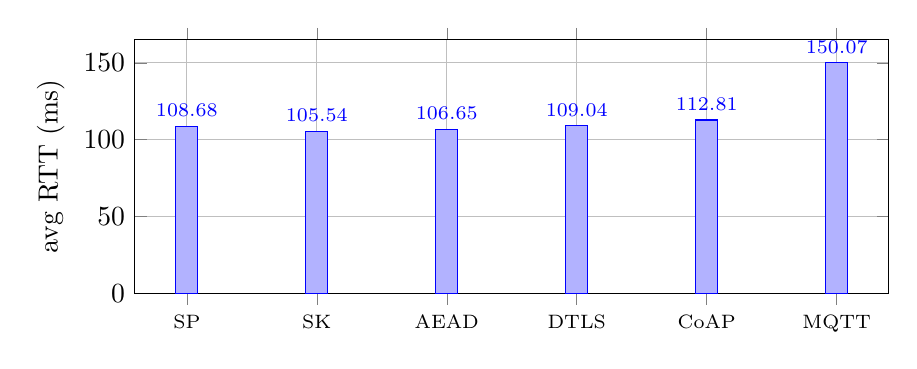
\begin{tikzpicture}
\begin{axis}[
  ybar,
  bar width=8pt,
  width=0.92\linewidth,
  height=4.8cm,
  ymin=0,
  ylabel={avg RTT (ms)},
  symbolic x coords={SP,SK,AEAD,DTLS,CoAP,MQTT},
  xtick=data,
  xticklabel style={font=\scriptsize},
  nodes near coords,
  every node near coord/.append style={font=\scriptsize},
  enlarge x limits=0.08,
  grid=major
]
\addplot coordinates {(SP,108.676) (SK,105.536) (AEAD,106.654) (DTLS,109.040) (CoAP,112.805) (MQTT,150.072)};
\end{axis}
\end{tikzpicture}

\vspace{2mm}
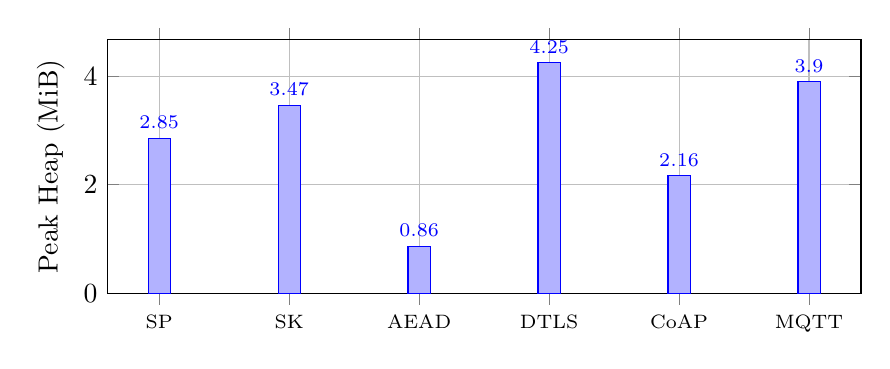
\begin{tikzpicture}
\begin{axis}[
  ybar,
  bar width=8pt,
  width=0.92\linewidth,
  height=4.8cm,
  ymin=0,
  ylabel={Peak Heap (MiB)},
  symbolic x coords={SP,SK,AEAD,DTLS,CoAP,MQTT},
  xtick=data,
  xticklabel style={font=\scriptsize},
  nodes near coords,
  every node near coord/.append style={font=\scriptsize},
  enlarge x limits=0.08,
  grid=major
]
\addplot coordinates {(SP,2.851) (SK,3.467) (AEAD,0.859) (DTLS,4.250) (CoAP,2.164) (MQTT,3.898)};
\end{axis}
\end{tikzpicture}
\caption{跨国受限网络下 RTT/峰值内存对照（SP=纯模式，SK=分包模式）}
\label{fig:c4-cross-core}
\end{figure}

\subsection{相对增益量化}
表~\ref{tab:c4-relative-gain} 给出组合数独协议相对 DTLS 与 MQTT/TLS 的增益。结果显示：组合数独协议相对 DTLS 的 RTT 优势有限（0.33\% 与 3.21\%），内存降幅分别为 32.92\% 与 18.42\%；相对 MQTT/TLS 的 RTT 优势分别为 27.58\% 与 29.68\%，内存降幅分别为 26.87\% 与 11.06\%。

\begin{table}[H]
\centering
\small
\caption{纯模式与分包模式相对 DTLS 与 MQTT/TLS 的跨国中位数增益}
\label{tab:c4-relative-gain}
\begin{tabularx}{\linewidth}{l>{\centering\arraybackslash}X>{\centering\arraybackslash}X>{\centering\arraybackslash}X>{\centering\arraybackslash}X}
\toprule
方案 & RTT 相对 DTLS & RTT 相对 MQTT & 内存相对 DTLS & 内存相对 MQTT \\
\midrule
纯组合数独 & +0.33\% & +27.58\% & +32.92\% & +26.87\% \\
6bit分包组合数独 & +3.21\% & +29.68\% & +18.42\% & +11.06\% \\
\bottomrule
\end{tabularx}
\end{table}

\subsection{开销与时延权衡}
图~\ref{fig:c4-overhead-rtt-tradeoff} 展示开销比与平均 RTT 的平面分布。纯组合数独位于高开销、同量级时延区域；6bit分包组合数独向低开销方向移动，同时保持 RTT 不劣于 DTLS，体现了两种模式在外观混淆强度与带宽效率之间的不同取舍。

\begin{figure}[!t]
\centering
\small
\begin{tikzpicture}
\begin{axis}[
  width=0.90\linewidth,
  height=6.0cm,
  xlabel={overhead ratio},
  ylabel={avg RTT (ms)},
  xmin=0.9, xmax=5.4,
  ymin=100, ymax=155,
  grid=major,
  legend style={at={(0.98,0.98)},anchor=north east,font=\scriptsize}
]
\addplot[only marks, mark=*, mark size=2.7pt] coordinates {(5.1813,108.676)};
\addlegendentry{纯组合数独}
\addplot[only marks, mark=square*, mark size=2.6pt] coordinates {(1.7389,105.536)};
\addlegendentry{6bit分包组合数独}
\addplot[only marks, mark=triangle*, mark size=2.8pt] coordinates {(1.1406,106.654)};
\addlegendentry{纯 AEAD}
\addplot[only marks, mark=diamond*, mark size=2.8pt] coordinates {(2.3279,109.040)};
\addlegendentry{DTLS}
\addplot[only marks, mark=o, mark size=2.6pt] coordinates {(1.0859,112.805)};
\addlegendentry{CoAP(UoT)}
\addplot[only marks, mark=star, mark size=3.0pt] coordinates {(2.4949,150.072)};
\addlegendentry{MQTT/TLS}
\end{axis}
\end{tikzpicture}
\caption{跨国受限网络下纯组合数独与 6bit分包的开销-时延权衡}
\label{fig:c4-overhead-rtt-tradeoff}
\end{figure}

\section{协议识别、类别恢复与主动攻击验证}
\subsection{被动侧写实验设置}
协议识别实验使用 5 轮采样，每轮 800 条消息、256B 负载、无填充。BCI 类别恢复实验构造四类负载（MI-left:80B、MI-right:82B、Blink:84B、Rest:86B），每类重复 3 轮；主报告比较三种模式：MQTT/TLS 对照、纯组合数独无填充、纯组合数独填充（20--45B 随机填充）。为补充跨协议与模式对照，本文在相同特征空间与留一法最近质心判定标准下，对 CoAP、纯 AEAD 与 6bit分包组合数独（prefer\_entropy）进行了统一复算（每协议每模式 $n=12$）。

DPI 对照实验中，组合数独 ASCII 样本由提示字节池与填充字节池按概率混合生成（提示概率 0.82），并与随机二进制样本比较可打印比例和规则分类标签。

\subsection{被动侧写结果}
侧写结果表明：协议识别准确率为 96.67\%（29/30），唯一误判来自纯组合数独与 6bit分包组合数独的一次互混；在类别恢复指标上，MQTT/TLS、CoAP/UDP、纯 AEAD 与组合数独协议无填充模式均为 1.0000，纯组合数独在 20--45B 填充模式下降至 0.1667，6bit分包组合数独（prefer\_entropy）填充模式为 0.2500。两条填充路径均显著低于无填充对照，说明填充机制可有效削弱长度序列侧写的可学习性\cite{alwhbi2024encrypted,hou2024encmalware}。

\begin{algorithm}[H]
\small
\caption{BCI 类别侧写评估：无填充为 100\%，随机填充显著降低恢复率}
\label{alg:c4-sidechannel-eval}
\KwIn{模式集合 $\mathcal{M}$，每模式样本 $\mathcal{D}_m=\{(s_i,y_i)\}$，防护策略参数 $\Pi_m$}
\KwOut{恢复率 $R_m$ 与风险等级 $L_m$}
\ForEach{$m \in \mathcal{M}$}{
  从长度序列 $s_i$ 截取 128 维窗口并提取统计特征 $x_i$\;
  采用留一法最近质心分类得到预测标签 $\hat{y}_i$\;
  $R_m \leftarrow \frac{1}{N_m}\sum_{i=1}^{N_m}\mathbf{1}(\hat{y}_i=y_i)$\;
  \eIf{$R_m \ge 0.9$}{
    $L_m \leftarrow$ 高风险（类别语义可重建）\;
  }{
    \eIf{$R_m \le 0.4$}{
      $L_m \leftarrow$ 受控风险（侧写可学习性显著下降）\;
    }{
      $L_m \leftarrow$ 中风险\;
    }
  }
}
比较 $\Pi_m=\varnothing$ 与 $\Pi_m=\text{随机填充}$ 的 $R_m$ 变化，判定防护收益\;
\end{algorithm}

从攻击语义看，被动攻击者只需观察长度序列即可恢复类别；当恢复率接近 1 时，业务类别轨迹会直接暴露，进而放大意图泄露与针对性干预风险。在 BCI-IoT 场景中，该风险将直接削弱用户隐私与控制链路安全性\cite{alwhbi2024encrypted,kapitonova2022framework,meng2024adversarial}。

协议识别召回率与 BCI 类别恢复率分别见图~\ref{fig:c4-proto-recall-extended} 和图~\ref{fig:c4-sidechannel-dpi}。

\begin{figure}[!b]
\centering
\small
\begin{tikzpicture}
\begin{axis}[
  ybar,
  bar width=9pt,
  width=0.86\linewidth,
  height=3.35cm,
  ymin=0,
  ymax=1.05,
  ylabel={协议侧写召回率},
  symbolic x coords={SP,SK,AEAD,MQTT,CoAP,DTLS},
  xtick=data,
  xticklabel style={font=\scriptsize},
  nodes near coords,
  every node near coord/.append style={font=\scriptsize},
  enlarge x limits=0.10,
  grid=major
]
\addplot coordinates {(SP,1.0) (SK,0.8) (AEAD,1.0) (MQTT,1.0) (CoAP,1.0) (DTLS,1.0)};
\end{axis}
\end{tikzpicture}
\caption{协议识别召回率对照（SP=纯模式，SK=分包模式；含 MQTT、CoAP、纯 AEAD、DTLS）}
\label{fig:c4-proto-recall-extended}
\end{figure}

进一步地，本文从协议识别混淆矩阵计算了各协议召回率（每类样本 5 轮）。图~\ref{fig:c4-proto-recall-extended} 显示，MQTT/TLS、CoAP/UDP、纯 AEAD、DTLS 与纯组合数独的召回率均为 1.0000；仅 6bit分包组合数独为 0.8000（1 次误判为纯组合数独）。这说明多类对照路线的外观特征均可被分类模型稳定学习。DPI 对照中，组合数独 ASCII 模式可打印比例为 0.9834，被归为明文样式；TLS 二进制样本为 0.3838，被归为密文二进制样式，表明外观层可改变规则式流量标签。

\begin{figure}[!t]
\centering
\small
\begin{tikzpicture}
\begin{axis}[
  ybar,
  bar width=9pt,
  width=0.90\linewidth,
  height=5.0cm,
  ymin=0, ymax=1.05,
  ylabel={类别恢复率},
  symbolic x coords={MQTT,CoAP,AEAD,SNoPad,SPad,SKPad},
  xtick=data,
  xticklabels={MQTT,CoAP,AEAD,SNoPad,SPad,SKPad},
  xticklabel style={font=\scriptsize},
  nodes near coords,
  every node near coord/.append style={font=\scriptsize},
  enlarge x limits=0.08,
  grid=major
]
\addplot coordinates {(MQTT,1.0) (CoAP,1.0) (AEAD,1.0) (SNoPad,1.0) (SPad,0.1667) (SKPad,0.25)};
\end{axis}
\end{tikzpicture}
\caption{BCI 类别恢复率对照：SNoPad=无填充，SPad=纯组合数独填充，SKPad=6bit分包填充；随机填充显著降低恢复率}
\label{fig:c4-sidechannel-dpi}
\end{figure}
\FloatBarrier

\subsection{主动攻击与 MITM 可恢复性验证}
主动攻击实验均在受控单机环境中进行：重放场景先完成一次合法握手并记录客户端发往服务端的原始握手字节，随后在第二次连接中原样重放该字节流；篡改场景在握手首个写入字节上执行单比特翻转，模拟链路中间人篡改；资源探测场景持续发送超出 $\texttt{maxProbeBytes}$ 上界的无效探测数据，观察服务端是否在握手探测阶段提前终止。对于前述三类场景，只要服务端返回的错误类型分别命中 \texttt{ErrReplayDetected}、\texttt{SuspiciousError}、\texttt{ErrAuthFailed} 或 \texttt{ErrProtocolViolation}，或在超长探测下进入可疑路径，即判定防御成功。

TLS MITM 对照实验采用另一条验证链路：攻击者先构造受控 CA 与伪造服务端证书，在客户端与真实服务端之间建立中间人代理；随后客户端按固定次序发送类别序列，代理在完成 TLS 握手后直接读取明文行并提取其中的类别字段，再将业务转发至真实服务端。若攻击者观测到的类别序列与发送序列逐项一致，则说明链路虽然采用 TLS 加密，但在终止代理点仍可恢复业务语义。表~\ref{tab:c4-security-evidence} 汇总了各攻击场景的实施动作、服务端观测与最终结果。组合数独协议在重放、篡改、资源探测三类主动攻击下均触发拒绝路径；TLS MITM 对照的恢复率为 1.0，说明攻击者可逐条恢复业务类别序列，链路加密无法消除终止代理点的业务可见性\cite{wilkens2021passivetls}。

\begin{table}[H]
\centering
\small
\caption{主动攻击与 TLS-MITM 对照：组合数独拦截重放/篡改，MITM 可恢复业务类别}
\label{tab:c4-security-evidence}
\begin{tabular}{>{\raggedright\arraybackslash}p{1.8cm}>{\raggedright\arraybackslash}p{3.5cm}>{\raggedright\arraybackslash}p{5.0cm}>{\raggedright\arraybackslash}p{1.8cm}}
\toprule
场景 & 攻击过程 & 服务端观测与成功判据 & 结果 \\
\midrule
重放攻击 & 首次握手正常完成并记录客户端握手字节；第二次连接原样重放同一字节流 & 服务端重放缓存命中，返回 \texttt{ErrReplayDetected}；命中即判定防御成功 & 成功拦截 \\
篡改攻击 & 对握手首个写入字节执行单比特翻转，再继续完成后续握手发送 & 服务端在摘要、签名或消息格式校验阶段返回 \texttt{SuspiciousError}、\texttt{ErrAuthFailed} 或 \texttt{ErrProtocolViolation}；进入拒绝路径即判定防御成功 & 成功拦截 \\
资源探测 & 向服务端连续写入远超握手探测上界的无效字节流（80KB） & 服务端在 probe 阶段因超过 \texttt{maxProbeBytes} 进入可疑路径并返回 \texttt{SuspiciousError}；提前终止即判定防御成功 & 成功拦截 \\
TLS MITM 对照 & 中间人代理使用伪造证书终止 TLS，会后逐行读取并提取 \texttt{BCI\_CLASS} 字段，再转发至真实服务端 & 将攻击者观测序列与发送序列逐项比较；恢复率接近 1 判定业务类别可恢复 & 恢复率 1.0 \\
\bottomrule
\end{tabular}
\end{table}

\subsection{Fallback 适用场景仿真}
为验证 fallback 的工程可用性，本文构造主动探测流量重定向场景：攻击侧先发送可疑握手前缀，再继续发送后续探测字节；服务端在握手阶段识别为可疑流量后，停止真实会话建立流程，并将已读前缀与后续字节转发至诱饵服务。仿真流程与结果见表 \ref{tab:c4-fallback-sim}。

\begin{table}[H]
\centering
\small
\caption{fallback 仿真：可疑握手前缀被诱饵完整接收}
\label{tab:c4-fallback-sim}
\begin{tabular}{p{2.0cm}p{4.1cm}p{4.0cm}p{2.8cm}}
\toprule
阶段 & 输入或动作 & 观测结果 & 结论 \\
\midrule
S1 可疑触发 & 发送异常握手前缀“\texttt{BAD}” & 服务端返回可疑错误并进入 fallback 路径 & 真实会话未建立 \\
\midrule
S2 连续转发 & 攻击侧继续发送“\texttt{HELLO}” & 诱饵端收到连续字节“\texttt{BADHELLO}” & 已读字节未丢失 \\
\midrule
S3 诱饵响应 & 诱饵端返回“\texttt{ACK}” & 攻击侧收到“\texttt{ACK}”响应 & 外部行为与普通服务一致 \\
\bottomrule
\end{tabular}
\end{table}

该场景表明，fallback 机制用于降低异常路径的可区分性，其作用范围限于异常流量处置。探测流量仅获得诱饵通道反馈，不返回真实协议状态。作为对照，TLS/DTLS、MQTT/TLS 与 CoAP/DTLS 路径在标准实现中通常表现为告警、断链或超时，不提供协议级已读字节回落接口（详见表 \ref{tab:c3-fallback-compare}）\cite{rfc8446,rfc9147,mqtt311,rfc7252}。

\section{对照方案风险归因与组合数独协议的工程权衡}
结合协议机理与实证结果，第 4 章的对比结论可置于“安全属性与工程成本同步分配”的分析框架中解释。BCI 场景需要将隐私与安全要求前置到系统设计阶段\cite{kapitonova2022framework}，IoT 安全方案也必须兼顾敏感数据保护、资源约束与部署适配\cite{trabelsi2023iotaccess}。

需要强调的是，本文方案的价值在于把握手认证、会话加密与外观抗侧写放入同一协议状态机，并为每一项安全属性支付明确成本：协议引入数独编码、可逆外观映射和随机填充后，确实增加了编码复杂度与线长/带宽开销；但长度序列、可打印比例和 DPI 标签不再与业务类别保持简单对应。若威胁模型仅关注端到端机密性与完整性，DTLS/MQTT-TLS 的成熟生态仍更合适；当攻击者能够长期观察链路并利用长度、时序或 DPI 标签实施侧写时，组合数独外观层提供了主流安全隧道之外的额外防护维度。

\begin{itemize}
  \item \textbf{CoAP（UDP）}：协议语义建立在 UDP 之上\cite{rfc7252}，但在跨国受限链路中需通过 UoT 中继，原生 UDP 部署优势难以直接发挥。
  \item \textbf{DTLS}：具备标准化握手与会话保护\cite{rfc9147}，但在受限公网常依赖中继与代理，运维信任范围扩大。
  \item \textbf{MQTT/TLS}：生态成熟、工程复用高\cite{mqtt311,rfc8446,zheng2023mqtttamarin}，但长度与时序特征仍可被侧写模型稳定利用\cite{alwhbi2024encrypted,hou2024encmalware}。
  \item \textbf{纯 AEAD}：记录层机密性与完整性明确\cite{rfc5116}，但缺乏独立握手认证与新鲜性语义，抗重放能力依赖额外状态机。
  \item \textbf{组合数独协议}：通过握手防护、外观调控与资源控制实现联合优化；纯模式偏重混淆能力，分包模式偏重带宽效率。
\end{itemize}

因此，组合数独协议在 BCI-IoT 场景下可视为兼顾安全语义、资源约束与外观调控能力的可部署方案：相较纯 AEAD，安全语义更完整；相较 MQTT/DTLS，在被动侧写威胁下具有更强的外观对抗能力；代价是纯模式路径带宽开销较高、实现复杂度和标准化生态仍需扩展（见表~\ref{tab:c4-cross-region-main}、图~\ref{fig:c4-sidechannel-dpi}、表~\ref{tab:c4-security-evidence}）。

\section{有效性威胁与适用条件}
本文结果在下列条件内成立。
\begin{itemize}
  \item \textbf{外部有效性}：跨国实验基于单个公网节点，未覆盖全部地区与运营商网络。
  \item \textbf{统计有效性}：跨国重复次数为 3，适合趋势判断，不用于细粒度显著性检验。
  \item \textbf{模型有效性}：侧写模型以特征工程为主，未覆盖大规模深度时序模型上界。
  \item \textbf{原型有效性}：结论对应本文所实现的协议原型，若迁移到其他语言或实现框架，仍需重新评估。
\end{itemize}

\section{本章小结}
本章建立了实验设计、指标算法、攻击判定与结果解释的一致性链路。结果显示：在跨国受限网络中，组合数独协议的 RTT 与主流协议处于同量级，数据面内存低于 DTLS 与 MQTT/TLS；在安全与对抗方面，组合数独协议可稳定拦截重放与篡改，填充机制可显著降低类别侧写恢复率。综合来看，组合数独协议具备可量化、可复核、可部署的应用可行性。
